%=======================02-713 LaTeX template, following the 15-210 template==================
%
% You don't need to use LaTeX or this template, but you must turn your homework in as
% a typeset PDF somehow.
%
% How to use:
%    1. Update your information in section "A" below
%    2. Write your answers in section "B" below. Precede answers for all 
%       parts of a question with the command "\question{n}{desc}" where n is
%       the question number and "desc" is a short, one-line description of 
%       the problem. There is no need to restate the problem.
%    3. If a question has multiple parts, precede the answer to part x with the
%       command "\part{x}".
%    4. If a problem asks you to design an algorithm, use the commands
%       \algorithm, \correctness, \runtime to precede your discussion of the 
%       description of the algorithm, its correctness, and its running time, respectively.
%    5. You can include graphics by using the command \includegraphics{FILENAME}
%
\documentclass[11pt]{article}
\usepackage{amsmath,amssymb,amsthm}
\usepackage{tikz}
\usetikzlibrary{arrows,positioning, calc}
\tikzstyle{vertex}=[draw,fill=black!15,circle,minimum size=20pt,inner sep=0pt]
\usepackage{graphicx}
\usepackage[margin=1in]{geometry}
\usepackage{fancyhdr}
\usepackage{mathtools}
\usepackage{placeins}
\usepackage{listings}
\usepackage{color}
\usepackage{forest}
\usepackage{tikz}

\definecolor{dkgreen}{rgb}{0,0.6,0}
\definecolor{gray}{rgb}{0.5,0.5,0.5}
\definecolor{mauve}{rgb}{0.58,0,0.82}

\lstset{frame=none,
  language=Java,
  aboveskip=3mm,
  belowskip=3mm,
  showstringspaces=false,
  columns=flexible,
  basicstyle={\small\ttfamily},
  numbers=none,
  numberstyle=\tiny\color{gray},
  keywordstyle=\color{blue},
  commentstyle=\color{dkgreen},
  stringstyle=\color{mauve},
  breaklines=true,
  breakatwhitespace=true,
  tabsize=3
}

\setlength{\parindent}{0pt}
\setlength{\parskip}{5pt plus 1pt}
\setlength{\headheight}{13.6pt}
\newcommand\question[2]{\vspace{.25in}\hrule\textbf{#1 #2}\vspace{.5em}\hrule\vspace{.10in}}
\renewcommand\part[1]{\vspace{.10in}\textbf{(#1)}}
\newcommand\algorithm{\vspace{.10in}\textbf{Algorithm: }}
\newcommand\correctness{\vspace{.10in}\textbf{Correctness: }}
\newcommand\runtime{\vspace{.10in}\textbf{Running time: }}
\pagestyle{fancyplain}
\lhead{\textbf{\NAME}}
\chead{\textbf{HW\HWNUM}}
\rhead{\today}
\begin{document}\raggedright
%Section A==============Change the values below to match your information==================
\newcommand\NAME{Sean Connor (443-414-5111)}  % your name
\newcommand\HWNUM{3}              % the homework number
%Section B==============Put your answers to the questions below here=======================
\question{Q1}{}
If $L_1 \leq_p L_2$, then there exists a function $f$ such that:
\begin{equation*}
x \in L_1 \iff f(x) \in L_2
\end{equation*} 
and if $L_2 \leq_p L_3$, then there exists a function $g$ such that:
\begin{equation*}
x \in L_2 \iff f(x) \in L_3
\end{equation*} 
where $f$ and $g$ are polynomial-time computable functions. Since both are polynomial-time computable, we can combine $f$ and $g$ (i.e. perform a composition of $f$ and $g$) to reduce $L_1$ to $L_3$, done as follows:
\begin{equation*}
x \in L_1 \iff g(f(x)) \in L_3
\end{equation*}
$g(f(x))$ is polynomial-time computable. Thus, $L_1 \leq_p L_3$.

\question{Q2}{}
If a graph has a clique of size $n$, then each vertex in the clique is adjacent to each other $n-1$ vertices in the clique. A vertex chosen at random has a color, and the other $n-1$ vertices each have a different color since they are all adjacent to one another. See Figure 1.

\begin{figure}[!htpb]
\centering
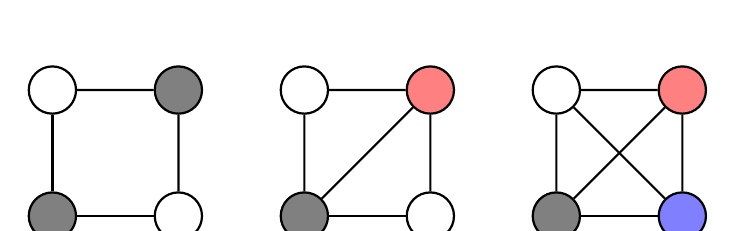
\begin{tikzpicture}
  [scale=.8,auto=left,every node/.style={circle, draw=black, thick, minimum width = 6mm}]
  \node [fill=black!50] (A) at (0,0) {};
  \node (B) at (0,2)  {};
  \node (C) at (2,0)  {};
  \node [fill=black!50] (D) at (2,2) {};
  
  \node [fill=black!50] (AA) at (4,0) {};
  \node (BB) at (4,2)  {};
  \node (CC) at (6,0)  {};
  \node [fill=red!50] (DD) at (6,2) {};
  
  \node [fill=black!50] (AAA) at (8,0) {};
  \node (BBB) at (8,2)  {};
  \node [fill=blue!50] (CCC) at (10,0)  {};
  \node [fill=red!50] (DDD) at (10,2) {};
  
  \path [-] [thick]
  (A) edge (B)
  (A) edge (C)
  (D) edge (B)
  (D) edge (C)
  
  (AA) edge (BB)
  (AA) edge (CC)
  (DD) edge (BB)
  (DD) edge (CC)
  (AA) edge (DD)
  
  (AAA) edge (BBB)
  (AAA) edge (CCC)
  (DDD) edge (BBB)
  (DDD) edge (CCC)
  (BBB) edge (CCC)
  (AAA) edge (DDD);               

\end{tikzpicture}
\caption{The left square is clique size two and requires two colors. The middle square is clique size three and requires three colors. The right square is clique size four and requires four colors.}
\end{figure}

Thus, at least n colors are required. A graph cannot be more connected than in the case of a clique, and thus $n$ is the minimum number of colors required, and not $n+1$, $n+2$, etc. Of course, there can be more colors required than the size of the maximal clique $n$, as shown in Figure 2.

\begin{figure}[!htpb]
\centering
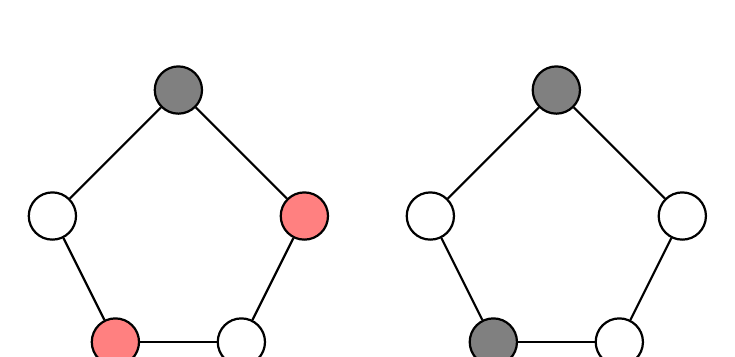
\begin{tikzpicture}
  [scale=.8,auto=left,every node/.style={circle, draw=black, thick, minimum width = 6mm}]
  \node (A) at (0,2) {};
  \node [fill=red!50] (B) at (1,0)  {};
  \node (C) at (3,0)  {};
  \node [fill=red!50] (D) at (4,2) {};
  \node [fill=black!50] (E) at (2,4) {};
  
  \node (AA) at (6,2) {};
  \node [fill=black!50] (BB) at (7,0)  {};
  \node (CC) at (9,0)  {};
  \node (DD) at (10,2) {};
  \node [fill=black!50] (EE) at (8,4) {};
  
  \path [-] [thick]
  (A) edge (B)
  (B) edge (C)
  (C) edge (D)
  (D) edge (E)
  (E) edge (A) 
  
  (AA) edge (BB)
  (BB) edge (CC)
  (CC) edge (DD)
  (DD) edge (EE)
  (EE) edge (AA);        

\end{tikzpicture}
\caption{The left pentagon has a maximal clique size of two, but requires three colors. The right pentagon does not satisfy the requirements.}
\end{figure}

\newpage

\question{Q3}{}
Here we show that the Efficient Recruiting problem (\textit{ER}) is NP-complete (NPC). To show this, we must show that \textit{ER} is NP, and that \textit{ER} is NP-hard.

First, we show that \textit{ER} is NP by verifying a certificate in polynomial time. This is easy to do - simply check that $m$ coaches is less than or equal to $k$, and then iterate through $n$ sports and $m$ coaches to see if all sports are covered. This is polynomial time O($mn$) and so \textit{ER} is NP.

Next, we show that \textit{ER} is NP-hard by showing that \textit{SET-COVER} $\leq_p$ \textit{ER}, since \textit{SET-COVER} is NPC. This can be done in a manner similar to \textit{HAM-CYCLE} $\leq_p$ \textit{TSP} from the text.

$A$ is an instance of \textit{SET-COVER} where there are subsets of a set $S=\{x_1,x_2, \dots ,x_n\}$.

$A'$ is an instance of \textit{ER} where each subset is a coach and each element of a set $S$ is a sport. We can show that \textit{ER} has a subset cover if and only if there are k or fewer subsets in $A'$ (counselors) that cover the items (sports) in set $S$. Since \textit{ER} has a subset cover and can be shown in polynomial time, we can say that \textit{ER} is NP-hard. 

Since \textit{ER} is NP and NP-hard, \textit{ER} is also NPC.

\question{Q4}{}
Here we show that the Diverse Subset problem \textit{DS} is NPC. 

First, verify a certificate in polynomial time to show that \textit{DS} is NP. This can be easily achieved by simply checking that there are $k$ or more elements in the certificate subset and then verifying that no customers in the subset ever bought the same product. This can be achieved in O($mn$) time, where $m$ is the number of items and $n$ is the number of customers in the subset. O($mn$) is polynomial time, and so \textit{DS} is NP.

Next, we need to show that \textit{DS} is NP-hard by showing \textit{IS} $\leq_p$ \textit{DS}.

\begin{figure}[!htpb]
\centering
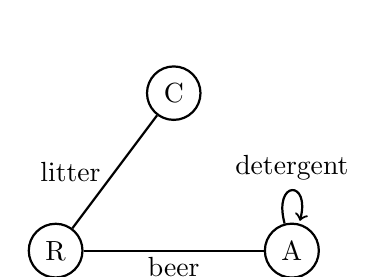
\begin{tikzpicture}
  \node (R) [circle, draw=black, thick, minimum width = 6mm] at (0,0) {R};
  \node (A) [circle, draw=black, thick, minimum width = 6mm] at (3,0) {A};
  \node (C) [circle, draw=black, thick, minimum width = 6mm] at (1.5,2) {C};

  
  \path [-] [thick]
  (R) edge node [yshift=-6pt]{beer} (A)
  (R) edge node [xshift=-16pt]{litter} (C)
  (A) edge [loop above] node {detergent} (A);
 

\end{tikzpicture}
\caption{Graph representation of Table 1 from prompt.}
\end{figure}

To show the reduction, let's first phrase the problem as a decision question. ``Given an $m \times n$ array as defined in the prompt and a number $k \leq m$, is there a subset of at least $k$ customers that is diverse?''

Construct a graph $G'$ which is an instance of $G$ from \textit{IS}. Each vertex in $G'$ represents a customer and each edge in $G'$ represents a product. Note that there can be multiple edges between vertices, and also edges pointing to the same vertex. We can show that $G'$ has a diverse subset of size $k$ if and only if there is an independent set of at least size $k$. Since there is an independent set, we can say that \textit{DS} is NP-hard.

Since \textit{DS} is NP and NP-hard, \textit{DS} is also NPC.

From the example in Table 1 in the prompt, we construct a graph as shown in Figure 3. Alanis and Chelsea form an independent set, as they have never purchased the same product and there is no edge between them. Thus, Alanis and Chelsea form a diverse set.

\end{document}









